\section{Ripple}
We live in an era we where we can have news from all around the globe nearly instantly. Despite being able to communicate overseas easily we still struggle to transfer money quickly. Ripple's goal is to enable money transfers as fast as we can exchange information. To achieve this, Ripple aims at connecting people through a network and to use this network so that money transfers from one user to another can be executed rapidly. 
\subsection{The Ripple Network}
Based on an IOweYou credit network, Ripple network can be visualized as a directed graph where the vertices are wallets and the edges represent the credit link between those wallets. Wallets are used by entities (physical or moral) and attest the amounts this entity has in its possession. Non-negative weight on an edge from A to B indicates the amount that B owes to A. Ripple enable users to set a limit on the amounts that others owe to you. By default, the credit on a link is upper-bound by $\infty$ but the wallet owner (A in our example) can customize it. There can be several links between two wallets and each link between A and B handle different currencies. We have two types of currencies in the Ripple network: XRP that is the native currency and all other currencies that are also called issued currencies. All currencies on credit links are issued currencies. Moreover, each wallet has a non-negative amount of XRP that is used to pay fees for transactions and can also be used as a currency.

\begin{figure}[h!]
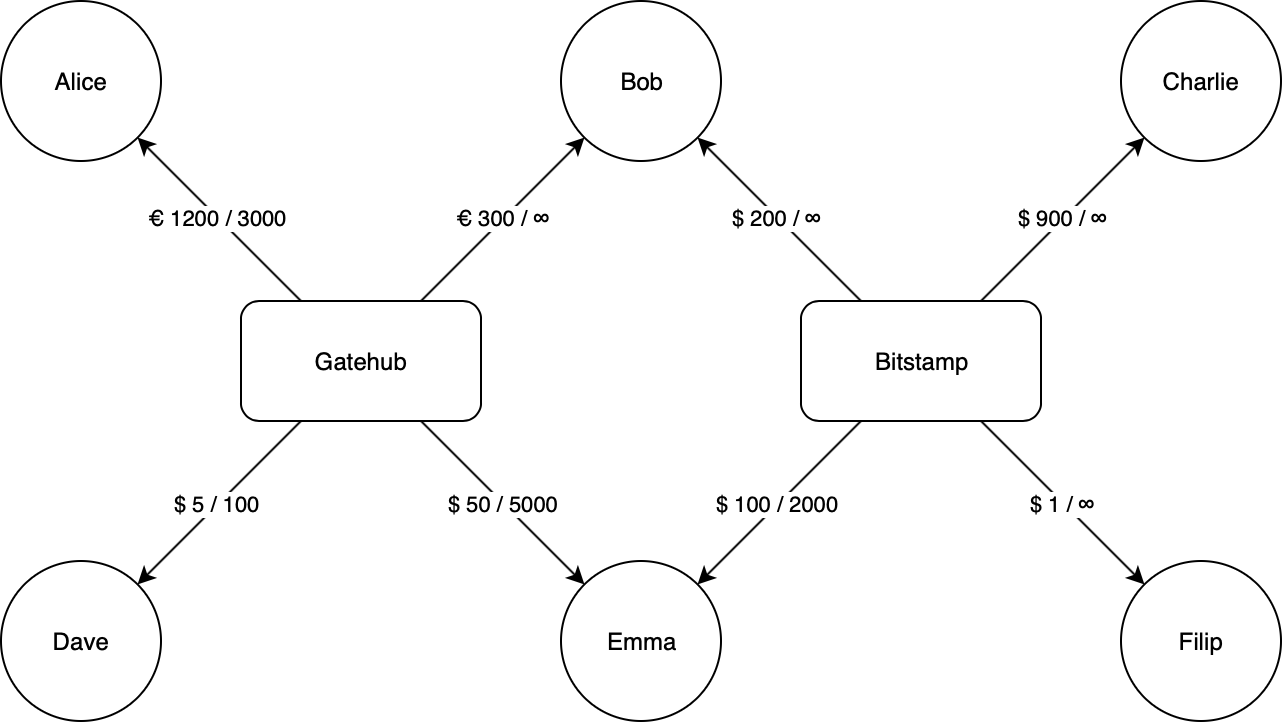
\includegraphics[width=\linewidth]{network.png}
\caption{Ilustrative example of the Ripple network}
\label{fig:network}
\end{figure}

Figure \ref{fig:network} depicts a possible fragment of the Ripple network. We have two gateways Bitstamp and Gatehub along with 6 users. Here, the credit link Gatehub $\rightarrow$ Alice denotes that Gatehub owes Alice 1200 EUR, and such credit is bounded by 3000 EUR. The credit link Bitstamp $\rightarrow$ Charlie tells us that Bitstamp owes Charlie 900 USD, and there is no upper limit on this credit link.

\subsection{Transactions}
There are two types of transaction in the Ripple network: direct XRP-payments and path-based transactions.

A direct XRP payment enables two wallets to pay each other even if they are not connected in the Ripple network. Basically, the XRP balance of the wallets is debited (and respectively credited) with the amount to transfer. As the name suggests that this type of transaction only involves XRP. 

All other currencies are exchanged over path-based transactions. Those transactions use a path of credit links that connects the sender to the receiver in order to make the transfer. Ripple has no way to enforce path based payments. It only records the amounts owed by one wallet to one other. A payment from A to B is only possible if there is a path that connects A to B. Moreover, A can only make a successful IOU payment to B if the payment value falls within the credit balance allocated on this path. For a given transaction, the total amount can be split into several paths. This enables to make payments even if there is not a single path that has enough credit capacity. In our example of Figure \ref{fig:network}, let's assume that Dave wants to pay Filip 5 USD. A possible path would be Dave $\leftarrow$ Gatehub $\rightarrow$ Emma $\leftarrow$ Bitstamp $\rightarrow$ Filip. When the transactions succeed the credit links are updated. In our situation, the links Dave $\leftarrow$ Gatehub and Emma $\leftarrow$ Bitstamp are decreased by 5 USD whereas Gatehub $\rightarrow$ Emma and Bitstamp $\rightarrow$ Filip are increased by 5 USD.

The combination of direct XRP payments and path-based transactions is natively supported in the Ripple network and they are atomically executed as a whole thanks to the Ripple Consensus (see 2.5)

\subsection{Main actors}
In addition to standard wallets, there are wallets with special characteristics.
\begin{description}
\item[Gateway] A gateway is a well-known established business that aims to help new users to enter the ripple network in an authenticated manner. Gateways are the Ripple equivalent of banks in the physical world. Their wallets maintain high connectivity. A newly created Ripple wallet that does not initially trust any existing wallet can create a credit link to a gateway and thereby interact with the rest of the network before creating direct links to other wallets.
\item[Market Maker] A market maker is a wallet that receives a certain currency on one of its credit links and exchanges it for another currency on another credit link, charging a small fee. Market Makers enable transactions where senders and receivers hold different currencies.
\end{description}

\subsection{Main operations}
To compose a path from a sender to a receiver, there are two possible operations Rippling and Exchanging.
\begin{description}
\item[Rippling] Rippling is the process of moving debts. In the XRP Ledger, Rippling defines the redistribution of credit links amounts between multiple connected parties who have trust lines for the same currency. Rippling is an essential part of issued currencies because it allows users who don't have a credit link between them to send issued balances to each other using a passive third user who serves as an intermediary. Rippling only exist along the paths of a payment. Rippling can only occur between two credit links that belong to the same wallet and have credit in the same denomination.
\item[Exchanging] Exchanging is the process of converting one currency to another. A wallet that is willing to exchange one currency for another creates an exchange offer for this pair, this wallet will then be identified as a market maker. The typical exchange offers are from issued currencies to issued currencies (eg. USD/EUR). However, it is possible to offer exchanges from/to XRP. There are some path-based transactions that use exchanges offered by market markers involving XRP, then the transaction becomes sort of both path-based and 'direct' in the sense that is used both XRP and issued currencies.
\end{description}
Back to Figure \ref{fig:network}, we now have Alice that wants to pay 100 USD to Charlie. Alice only has credit links only in EUR, however, suppose Bob publishes an offer EUR/USD with a rate 1 USD = 0.9 EUR. Bob plays the role of a Market Maker and enables Alice to pay Charlie by spending 90 EUR. The links are updated as follow: Alice $\leftarrow$ Gatehub is decreased by 90 EUR, Gatehub $\rightarrow$ Bob is increased by 90 EUR, Bob $\leftarrow$ Bitstamp is increased by 100 USD and finally Bitstamp $\rightarrow$ Charlie is increased by 100 USD.
Notice that the links of Gatehub and Bitstamp are shifted respectively by 90 EUR and 100 USD due to Rippling. Bob is a Market Marker in this situation.

\subsection{Nodes and Consensus}
The XRP network presented in the previous subsection is contained in a ledger. Every few seconds the XRP ledger has a new version which increments the index of the ledger by one. To operate properly and make the ledger progress with the arrival of new transactions, the XRP ledger relies on a set of servers. When a wallet wants to make a payment, it sends the transaction information to one server and it needs to operate according to rules so that the transaction may be applied and executed in the next version of the ledger.

The peer-to-peer XRP ledger network consists of many independent servers that receive and process transactions. The servers need to relay these candidates transactions to the other servers so that it can be applied to the ledger and validated by the validators. The server software that powers the XRP Ledger is called rippled\cite{rippled}, it enables servers to communicate in a peer-to-peer network.
The XRP ledger servers are also called nodes. There are two main types for nodes in rippled:
\begin{description}
\item[Stock server] Follows the network with a local copy of the ledger, propagates transactions and answers questions about the ledger.
\item[Validating server] validator for short - Participates in Consensus, a process designed to accept or deny a transaction based on some rules (and does everything a stock server does)
\end{description}
Servers propose transactions to apply to the current version of the ledger, this could lead to different versions with different content for the same ledger index. Of the many candidates, only one can become validated and thus there is only one valid ledger for each index. When a set of transactions can be applied to the ledger, and that validator has agreed on this set a new version of the ledger is created and it is marked as $validated$. In a perfect scenario, each new transaction would be known to each node allowing each to consider the same set of transactions to apply to the current version of the ledger. However, transactions take time to propagate and servers are not aware of all transactions. To answer this problem, the XRP Ledger uses a process called Consensus to ensure that all nodes have the same last version of the validated ledger.
\vspace{\baselineskip}

In section 2 we present some background about Ripple. Our work is described in section 3. The limitations to our work are explained in the next section. Finally, we give a conclusion and further steps in section 5 and 6.

%Consensus comes in three steps:
%%\item[Deliberation] Nodes iteratively propose a set of transactions to apply to the prior ledger. Nodes receive proposals from other trusted nodes and adjust their set of transactions. When a node believes enough proposals agree, it applies the corresponding transactions to the prior ledger according to the ledger protocol rules. It then issues a validation for the generated ledger.
%\item[Validation] Nodes decide if they fully validate a ledger, given the validations received from trusted nodes. Once the needed amount of validations for the same ledger is reached, that ledger is fully validated and become irreversible.
%\item[Preferred Branch] Nodes determine the most popular working branch of ledger history. There could be conflicts due to asynchrony, network difficulties and nodes could validate different ledgers for the same index. The nodes use the ledger ancestry of trusted validations to get back to the network’s preferred branch.
%\end{description}